\documentclass[french,12pt]{report}
\usepackage{babel}
\usepackage{a4}
\usepackage{amsmath}
\usepackage{graphicx}

\begin{document}
\sloppy

\begin{titlepage}
\begin{center}

%\setlength{\unitlength}{1in}
%\begin{picture}(0,0)
%   \put(-4.3,-10){\includegraphics{fond4.eps}}
%\end{picture}

.
\vspace{5.3cm}

\Huge \bf {POULE}

\vspace{2cm}

\large
\bf {Rapport d'avancement}

\vspace{2cm}

\mdseries
\begin{tabular}{l r}
Nicolas \textsc{Metais} & Jean-Daniel \textsc{Michaud} \\
Jonathan \textsc{Mimouni} & Francois \textsc{Morlot}
\end{tabular}

\vspace{2cm}
Le \today

\end{center}
\end{titlepage}

\strut\thispagestyle{empty}
\vfill
\pagebreak
\setcounter{page}{1}
\tableofcontents
\pagebreak


\section*{Introduction}
\addcontentsline{toc}{chapter}{Introduction}
\markboth{\uppercase{Introduction}}
{\uppercase{Introduction}}

Ce document  est le rapport  d'avancement de \emph{Poule}.  Il propose
aux souteneurs de  ce projet de d\'ecrire ce qui a  \'et\'e fait et ce
qu'il reste \`a faire.

\chapter {Cahier des charges}

Cette partie est le  cahier des charges  du projet \emph{Poule}.  Il a
pour  principale fonction  de d\'efinir  les limites  de \emph{Poule},
ainsi que de d\'efinir  ses principales fonctionnalit\'es. Nous sommes
rest\'es  d\'elib\'er\'ement flous  dans la  d\'efinition  de celui-ci
afin de ne  pas hypoth\`equer nos chances de  rendre un projet complet
et finalis\'e dans les temps.

Nous  pr\'eciserons aussi  dans  cette partie  les  d\'etails de  notre
organisation.  Ainsi la r\'epartition  des t\^aches  et l'organisation
temporelle sont pr\'esent\'ees dans la deuxieme partie.

\section{Sp\'ecifications}

Les  math\'ematiques sont  la base  de beaucoup  d'autres  sciences et
applications aussi  bien scientifiques que  commerciales. La physique,
la biologie ou encore la cryptographie, toutes ces sciences se servent
all\`egrement des math\'ematiques  pour formaliser et structurer leurs
th\'eories   fondamentales.  D\`es  l'apparition   de  l'informatique,
domaine qui  comme son  nom l'indique a  pour base  l'information, les
ordinateurs  ont  \'et\'e  mis   \`a  contribution  pour  traiter  des
informations   purement  num\'eriques   en  premier   lieu   pour  les
universit\'es americaines.  Mais  tr\`es vite, les math\'ematiciens ce
sont apercus que les ordinateurs pouvaient bien plus que manipuler des
nombres, aussi grands soient-ils.

Les  calculs formels sont,  en effet,  parfois de  vrais casse-t\^etes
pour les math\'ematiciens m\^eme les plus chevronn\'es. Parfois tr\`es
compliqu\'es, ils sont sources d'erreurs et de pertes de temps. Ainsi,
utiliser   la   puissance   des   ordinateurs   coupl\'ee   \`a   leur
infaillibilit\'e semblait  naturelle.  Mais les choses ne  sont pas si
\'evidentes.   La   puissance  des   ordinateurs   provient  de   leur
simplicit\'e. Amen\'es \`a ne manipuler que des nombres, ils sont tout
\`a  fait  incapables  d'int\'egrer  des notions  de  formalisme.  Une
\'equation  semblant simplissime pour  un \^etre  humain ne  l'est pas
pour un ensemble  de fils et de commutateurs.  Voici un exemple simple
mais convainquant:
$$ f(x) = 2 * x $$

Pour un \^etre humain n'ayant pas oubli\'e ses cours du coll\`ege, que
cela  represente-t-il  ?  Une  fonction.  Une fonction  qui  prend  en
param\`etre  un x  quelconque  et  qui a  pour  valeur le  param\`etre
multipli\'e   par  l'entier   2.    Pour  un   ordinateur,  que   cela
repr\'esente-t-il ? Une simple  cha\^ine de caract\`eres. Une cha\^ine
o\`u  tous  les  symboles  ont  une  m\^eme  signification.   $f$  est
\'equivalent  \`a $)$  qui lui  m\^eme  est \'equivalent  \`a $*$.  On
comprend pourquoi il sera difficile de faire comprendre \`a la machine
que $ f(3) = 6 $.

Le premier  compilateur fut \'ecrit en  avril 1957 par  John Backus et
son \'equipe. Il compilait le  langage \emph{FORTRAN}, mais cela a peu
d'importance. Ce qui  est important, c'est que pour  la premi\`ere fois
de  son histoire,  l'ordinateur \'etait  capable de  ``comprendre'' un
langage de  plus haut  niveau que le  simple assembleur,  reflet trait
pour trait, de son  architecture. Le domaine d'application du principe
des  compilateurs  est tr\`es  vaste.  Interpretation  de scripts,  de
fichiers de  configuration, de protocoles  de communication... partout
o\`u l'information est repr\'esent\'ee  sous forme de texte \'ecrit et
lisible  par un  \^etre  humain  et devant  \^etre  manipul\'ee par  un
ordinateur. C'est le  cas du calcul formel o\`u la  base du calcul, la
formule,  doit \^etre integr\'ee  et manipul\'ee  par la  machine.  Le
principe d'un  compilateur est assez  simple. A partir  d'une entr\'ee
(du texte) et d'une grammaire,  le compilateur construit un arbre. Cet
arbre est ensuite facilement manipul\'e par la machine pour produire le
r\'esultat attendu,  que se soit  pour le traduire en  langage machine
(compilation), pour le parcourir  et le r\'eduire (calcul num\'erique)
ou  le   r\'eduire  et   le  transformer  (calcul   num\'erique).  Ces
op\'erations sont les objectifs du projet \emph{Poule}.

\section{But}

Notre but  est de r\'ealiser un  logiciel de calcul  formel capable de
manipuler  une  formule entr\'ee  par  l'utilisateur et  d'\'effectuer
diff\'erents  calculs de mani\`ere  formelle. De  m\^eme, \emph{Poule}
sera capable  d'\'effectuer des  calculs num\'eriques sur  des nombres
arbitrairement grands, la capacit\'e ne serait alors limit\'ee que par
les  caract\`eristiques   de  la  machine.    L'analyse  de  fonctions
math\'ematiques pourra  \^etre continu\'ee d'une  visualisation par un
module  de  trac\'e  de  courbes.  Afin  de  rendre  l'utilisation  de
\emph{Poule}  plus intuitive,  une interface  permettra la  saisie des
donn\'ees et l'affichage des  formules. Enfin, un langage de scripting
pourrait   venir  compl\`eter  les   fonctionnalit\'es  du   projet  et
permettrait l'automatisation de certaines t\^aches.

\section{Module formel}

\emph{Poule}  est avant  tout une  plateforme de  calcul  formel.  Son
environnement   permettra  de   manipuler   des  entit\'es   abstraites
d\'efinies par leur appartenance \`a un domaine de d\'efinition.


Constituant  la  base  du   module  calcul  formel,  les  domaines  de
d\'efintion feront l'objet d'un contr\^ole rigoureux qui pr\'ec\'edera
tout calcul.

\subsection{Le contr\^ole de types}

Le contr\^ole  de type constitue la  premi\`ere \'etape d'\'evaluation
d'une expression.


Toutes les entit\'es de \emph{Poule} sont typ\'ees:
\begin{itemize}
\item les valeurs num\'eriques, par d\'efinition
\item les  variables, qui appartiennent  obligatoirement \`a un  et un
  seul domaine de d\'efinition
\item  les op\'erateurs,  qui manipulent  des op\'erandes  typ\'ees et
renvoient des expressions typ\'ees
\item les  fonctions dont  les arguments et  la valeur de  retour sont
typ\'es
\item les types abstraits d\'efinis par l'utilisateur, puisqu'ils sont
form\'es \`a partir de types pr\'eexistants
\end{itemize}

Ce  rigoureux  contr\^ole  du   typage  \`a  pour  but  d'assurer  une
coh\'erence des r\'esultats, de  renforcer la stabilit\'e du projet et
d'apporter un confort \`a l'utilisateur  qui en cas d'erreur de typage
verra  son  op\'eration abandonn\'ee  avant  le  d\'ebut des  calculs,
\'eventuellement co\^uteux en temps.

Une fois le contr\^ole de  type effectu\'e, le moteur de calcul formel
de \emph{Poule} met en place ces diff\'erentes fonctionnalit\'es.

\subsection{Calcul arithm\'etique sur les entit\'es formelles}

La  fonctionnalit\'e de base  du projet  est le  calcul arithm\'etique
avec les operateurs usuels (+, -, *, /) sur des entit\'es formelles.

\paragraph{}
{\bf Exemple: }
\begin{math}
  (x + x + 2)
\end{math}
{\it  est traduit en } 
\begin{math}
  (2 \times x + 2)
\end{math}

\subsection{Factorisation/D\'eveloppement}

La  factorisation  d'une expression  permet  de traduire  l'expression
originale sous  forme d'un  produit d'expressions plus  simples. Cette
fonctionnalit\'e sera  utile pour  les \'etudes de  signe, ou  pour la
r\'esolution d'\'equations.

L'op\'eration   compl\'ementaire    est   le   d\'eveloppement   d'une
expression.

Il est possible de  r\'ealiser une factorisation ou un d\'eveloppement
partiel  en   pr\'ecisant  la   variable  par  rapport   \`a  laquelle
l'op\'eration doit \^etre r\'ealis\'ee.
    
\paragraph{}
{\bf Exemples: }
\begin{enumerate}
\item
  \begin{math}
    fact ((x + 1) * (2 * x + 4))
  \end{math}
  {\it  est traduit en }
  \begin{math}
    (2 \times (x + 1) \times (x + 2))
  \end{math}
\item
  \begin{math}
    expand (x * (5 * y + z) / 7, x)
  \end{math}
  {\it  est traduit en }
  \begin{math}
    (\frac{5 \times x \times y + x \times z}{7})
  \end{math}
\item
  \begin{math}
    fact (expand ((x + 1) * (x + 1))) 
  \end{math}
  {\it  est traduit en }
  \begin{math}
    (x + 1)^{2}
  \end{math}
\end{enumerate}

\subsection{Simplification d'expressions}

La  simplification  d'une  expression  consiste  en  son  \'evaluation
formelle (permettant de simplifier par exemple y - y en 0), puis en sa
factorisation, et  enfin en la simplification  en \'el\'ements neutres
des  expressions  mettant en  relation  une  loi  de composition,  une
op\'erande et son inverse par la  loi de composition (par exemple, 3 *
x / 3 devient x).  Plusieurs algorithmes de simplification existent et
se combinent  tels les simplifications  par termes ou  facteurs. Assez
simples   et   donc   assez   rapides,  ils   donnent   d'assez   bons
r\'esultats.   Mais  il   est   important  de   noter  que   certaines
simplifications  faites  naturellement  \`a  la  main  peuvent  \^etre
dangereuses si elles sont effectu\'ees systematiquement.

Il est aussi int\'eressant  de remarquer que certaines simplifications
donnent des r\'esultats diff\'erents  selon le domaine de d\'efinition
des variables.

\paragraph{}
{\bf Exemples: }
\begin{enumerate}
\item
  \begin{math}
    \sqrt {x^{2}} | x > 0
  \end{math}
      {\it  se simplifie en } x
\item
  \begin{math}
    \sqrt {x^{2}} | x < 0
  \end{math}
  {\it  se simplifie en } -x
\end{enumerate}


\subsection{Substitution de variables}

Il est possible  de substituer une variable par  une valeur, une autre
variable ou une expression.

La substitution d'une  variable par une autre variable  n'est pas sans
rappeler l'alpha-r\'eduction  du lambda-calcul. Cette fonctionnalit\'e
sera se montrer utile  lors de la manipulation d'expressions contenant
des variables libres.

\paragraph{}
{\bf Exemple: }
\begin{math}
  (ln(x) + y) | x = 2 
\end{math}
 and 
\begin{math}
  y = ln(z)
\end{math}
{\it  est traduit en } 
\begin{math}
  (ln(2 \times z))
\end{math}


\subsection{Evaluation d'expressions}

L'\'evaluation d'une expression consiste  en la substitution de toutes
les variables de l'expression  par une valeur respectant l'ensemble de
d\'efinition de la variable, puis en son calcul alg\'ebrique.

\paragraph{}
{\bf Exemple: }
\begin{math}
  (sqrt(x) + y) / z | x = 5
\end{math}
and 
\begin{math}
  y = 1
\end{math}
and 
\begin{math}
  z = 2
\end{math}
{\it  s'\'evalue en } 
\begin{math}
  1.618 033 989
\end{math}

\subsection{R\'esolution de syst\`emes d'\'equations et d'in\'equations}

\emph{Poule} r\'esoud les \'equations  \`a une ou plusieurs inconnues.
Il permet \'egalement la r\'esolution des syst\`emes d'\'equations \`a
solutions r\'eelles et complexes.

Il est  possible de  pr\'eciser un intervalle  dans lequel  les racines
(valeurs   des  variables  qui   annulent  les   \'equations)  doivent
appartenir.

Toutes  ces  fonctionnalit\'es  sont  \'egalement  valables  pour  les
in\'equations et syst\`emes d'in\'equations.

\subsection{Calcul de d\'eriv\'ees}

Le moteur de calcul formel  de \emph{ Poule} offre la possibilit\'e de
calculer,   sous   sa  forme   factoris\'ee,   la  d\'eriv\'ee   d'une
fonction. \\Il est \'egalement possible:
\begin {itemize}
\item de calculer la d\'eriv\'ee d'une fonction en un point;
\item de pr\'eciser  la variable par rapport \`a  laquelle doit \^etre
calcul\'ee la d\'eriv\'ee, dans  le cadre d'une fonction \`a plusieurs
variables;
\item d'obtenir la d\'eriv\'ee n-i\`eme d'une fonction.
\item d'effectuer des calculs de Laplaciens, de rotationnels, ...
\end{itemize}


Evidement,   toutes  ces   fonctionnalit\'es  n\'ecessitent   que  les
fonctions utilis\'ees soient d\'erivables.


\subsection{Calcul de primitives et d'int\'egrales}

De  la  m\^eme fa\c{c}on  que  les  d\'eriv\'ees,  \emph{ Poule}  sait
calculer  les  primitives  d'une  fonction.  Il est  possible  de  lui
pr\'eciser la valeur de la constante d'int\'egration.


Li\'e au calcul de primitives, le calcul d'int\'egrales met en jeu des
r\`egles  plus fines  (comme la  reconnaissance d'une  fonction paire,
simplifiant  le r\'esulat).  D'autre part,  \emph{ Poule}  est capable
d'effectuer des  calculs sur des  int\'egrales impropres (int\'egrales
qui font intervenir  des bornes infinies, ou encore  une fonctions non
d\'efinies aux bornes ou en points de l'intervale \'etudi\'e).  Enfin,
l'imbrication  des  int\'egrales  permet  des  calculs  d'int\'egrales
doubles, triples, ...


\section{Module num\'erique}

\subsection{Calcul sur les flottants}

Cette partie regroupe toutes les differentes fonctions appel\'ees lors
de l'\'evaluation  num\'erique d'une formule.  On y trouve,  bien sur,
les  differents  operateurs($+$,$-$,$*$,$/$),  mais aussi  des  autres
fonctions     comme    log,     exponentiel    et     les    fonctions
trigonometriques.    Celles-ci   seront    calcul\'ees    \`a   partir
d'approximations. En effet, il serait interessant de pouvoir disposer
d'une  precision   variable.  On  ne  veut  pas   toujours  un  calcul
extremement  pr\'ecis, mais  il est  utile de  pouvoir  disposer d'une
precision  arbitrairement grande.  Cela nous  permettra  d'inserer des
algorithmes  de calcul de  $\pi$ et  de $e$  pour correspondre  \`a la
pr\'ecision demand\'ee.   Il faudra donc  un module de calcul  sur des
nombres   flottants    arbitrairement   grands,   un   d'approximation
num\'erique  de  formules  et   un  de  calcul  des  constantes  comme
$\pi$. Ces  fonctions devront  respecter une contrainte  de rapidit\'e
car elles  seront utilis\'ees tr\`es souvent. Par  exemple, pour faire
une integrale num\'erique, il faudra calculer des milliers de fois une
fonction complexe contenant elle-m\^eme plusieurs fonctions de calcul.

\subsection{Calcul sur les entiers}

Cette  partie regroupe  toutes  les operations  sp\'ecifiques sur  les
entiers.   En effet,  les operations  se rapprochent  de celles  sur les
flottants (sans  aucun chiffre  apres la virgule).  Il y a  donc, dans
cette  partie,  les  differentes  operations  arithmetiques.  On  peut
imaginer differents  tests de primalit\'e (par exemple  un test rapide
probabiliste  et  un  plus  lent  bas\'e sur  le  principe  du  crible
d'erathostene). De plus, on peut rajouter des fonctions de congruence,
de factorisation en facteurs premiers et quelques autres fonctions.


\section{Module graphique}

Le  module graphique  fait partie  des modules  qui ne  presentent \`a
priori que peu  d'interet au niveau de leur  programmation. Mais, tout
comme le module IHM, il a pour r\^ole "d'\'eclairer" l'utilisateur sur
le r\'esultat. En effet,  la trac\'e graphique permet \`a l'utilisateur
de visualiser \'enormement de choses en un seul coup d'oeil; ainsi une
fonction obscure comme par exemple
\begin{center}
\verb!integrate(exp(2*x^3 - 4) + 7) * cos (x)^3!
\end{center}

s'interpr\'ete  beaucoup mieux,  pour une  etude rapide,  sous  la forme
d'une courbe.  En effet la representation graphique en 2D d'une simple
fonction donne \`a tout bachelier une mine d'informations: Son allure,
ses racines simples, ...

Bien entendu, nous  avons pour objectif de d\'epasser  ce simple cadre
de  visualisation  en  2D.  Des  rendus 3D  permettant  de  visualiser
certaines courbes  sont prevus. De plus,  une certaine interactivit\'e
avec  le  module  graphique  est  envisageable.  La  possibilit\'e  de
d\'efinir  les bornes  pour le  calcul de  racines directement  sur le
graphe  ou le  calcul d'une  int\'egrale num\'erique  font  partie des
actions rendant le graphe plus dynamique.

\section{Module IHM}

L'Interface  Homme-Machine (\emph{IHM})  de \emph{Poule}  est,  \`a la
base,  constitu\'ee  du  terminal  classique  d'\emph{Unix}.  Celui-ci
permettra la lecture des  formules et des diff\'erents traitements \`a
y appliquer ainsi que  les ``commandes syst\`eme'' aff\`erentes \`a la
gestion de \emph{Poule}. Il  permettra aussi la sortie des r\'esultats
des  calculs   et  des   diff\'erents  messages  \`a   l'attention  de
l'utilisateur.

Produire une  belle interface,  haut en couleur  n'est pas le  but, ni
m\^eme un inter\^et  de ce projet. Malgr\'e tout,  il nous faut \^etre
pragmatique, l'\'ecriture  et la lecture  de formules math\'ematiques,
parfois longues et  complexes peut se transformer en  un vrai calvaire
sur les terminaux usuels  d'\emph{Unix}. C'est pourquoi une \emph{IHM}
graphique,  peut \^etre d'un  grand secours.  Mais comme  nous l'avons
dit, elle  ne doit pas monopoliser  notre temps et  nous emp\^echer de
developper les parties centrales  de notre projet. Ainsi, nous restons
d\'elib\`erement hypoth\'etique  sur l'avenir de  cette \emph{IHM}. Le
but sera  de mod\'eliser un projet  pouvant, si le  temps nous manque,
accepter plus tard un front-end graphique.

De quoi ce  module peut-\^etre constitu\'e ? D'une  part, et cela nous
semble  essentiel, d'une  fen\^etre graphique  capable  d'afficher les
diff\'erents signes math\'ematiques  composant les formules. Chiffres,
lettres, symboles d'int\'egration, etc ... Mais aussi d'un ensemble de
boutons accessibles  \`a la souris permettant la  simplification de la
saisie  de  formules.  Ainsi,  vouloir d\'efinir  l'int\'egral  de  la
fonction  exponentielle   de  borne   inferieure  \'egale  \`a   0  et
sup\'erieure \'egale \`a 1:
$$ \int_{0}^{1} e^x dx $$
se fera difficilement sur un terminal:
$$ \verb!integrate (exp(x), x, 0, 1)! $$
Mais beaucoup plus facilement gr\^ace \`a l'\emph{IHM}. Le proc\'ed\'e,
m\^eme s'il n'est pas rigide, pourra se pr\'esenter ainsi:


$$ \verb!clic sur le bouton d'integration! $$
$$ \verb!clic sur la fonction exponetielle! $$ 
$$ \verb!clic sur la variable x! $$
$$ \verb!entree manuelle des deux bornes! $$
$$ \verb!clic sur le bouton de calcul numerique! $$

On le  voit, l'\emph{IHM}, malgr\'e  son manque d'inter\^et  au niveau
d\'veloppement,  reste un  attribut essentiel  de  \emph{Poule}, c'est
pourquoi son int\'egration future devra \^etre prise en compte.

La mod\'elisation est la prochaine \'etape de notre travail. Bien nous
organiser  pour construire une  mod\'elisation \`a  la hauteur  de nos
amibtions est l'objectif courant.

\section{Sources d'informations}

Principalement  les livres  et  le net.  Notre  souteneur aussi,  Yann
Regis-Gianas. Mais nous envisageons de contacter les auteurs de COQ ou
FOC si le besoin s'en fait sentir.

\section{Internet}

\begin {itemize}
\item {ocaml.inria.fr}
\end {itemize}

\section{Livres}

Les principaux ouvrages sont:
\begin {itemize}
\item {Le calcul formel en pascal, d'Albert Levinas}
\item {Le calcul formel, de J. Davenport, Y. Siret et E. Tournier}
\end {itemize}

\pagebreak

\section{Conclusion}

Le grand  d\'efi de notre projet  ne tient pas en  la r\'ealisation de
toutes ces fonctionnalit\'es mais  avant tout en l'\'elaboration d'une
plateforme    de   calcul    formel   {\bf    extensible}    et   {\bf
intelligente}.  Par ``extensible'', nous  entendons qu'il  sera facile
d'int\'egrer   de   nouvelles   fonctionnalit\'es   au   projet.   Par
``intelligente'',  nous  entendons  que  \emph{  Poule}  sera  capable
d'apprendre de l'utilisateur. \\En effet, il sera possible d'enseigner
\`a \emph{ Poule} de nouvelles lois de simplification (par exemple:
\begin{math}
  {x^{a}} \times {x^{b}} = {x^{a+b}}
\end{math}
).  Toute la  puissance de  \emph{  Poule} sera  alors d'utiliser  ces
nouvelles r\`egles assimil\'ees au sein de ses fonctionalit\'es.

\chapter {Etat de l'art}

Les  logiciels de  calculs  formels existent  d\'ej\`a,  et n'ont  pas
attendu \emph{Poule}.  Les premiers  datent de 1960, avec l'apparition
du  LISP,  permettant  d\'ej\`a  des  integrations  formelles  et  des
d\'emonstrations de th\'eor\`emes.   Mais l'absence de standardisation
dans ce domaine et la distribution de logiciels sur des platformes peu
repandues ou  inconnues du grand-public (VAX-VMX ou  autres) n'ont pas
contribu\'e  au  developpement  de  cette  discipline.   Les  premiers
logiciels puissants  de calculs formels  sont les logiciels  REDUCE et
MACSYMA. Ils sont tous les deux \'ecrit en LISP et l'\'evolution de ce
languages, ainsi que sa  standardisation et son developpement on rendu
ces  deux  platformes  tr\`es  accessibles. Sur  micro-ordinateur,  au
milieu des ann\'ees 80, sont apparus des syst\`emes limit\'es tels que
muMATH et  son remplacant DERIVE. Enfin, plus  recemment sont apparues
des platformes compl\`etes et  puissantes et \'ecrit en C, MATHEMATICA
et MAPPLE.

\chapter {Infrastructure et choix des technologies}

Nous avons travaill\'e \`a quatre sur ce projet. Le temps imparti ayant
\'et\'e relativement  cours, nous avons d\'ecid\'e  de nous impliquer,
plus ou moins, dans toutes les  parties du projet. Ce qui nous permet,
\`a tous, d'avoir une vision d'ensemble.

\section{R\'epartition des t\^aches}

\includegraphics{GantVertical.ps}

\section {Environnement et langage de programmation}
La question du syst\`eme d'exploitaton ne s'est m\^eme pas pos\'ee. On a
choisi  le  syst\`eme  des  salles  machines de  l'\'ecole.  Quant  au
langage, c'est  cela qui a form\'e  le groupe, avant m\^eme  le sujet en
lui m\^eme. Cela fait plusieurs mois que nous avions d\'ecid\'e de faire
notre projet libre en OCaml.

\section {Compilation, autoconf et automake}
Pour compiler  notre projet, deux approches  \'etaient possibles, l'une
par  OCamlMakefile  et  l'autre  par Autoconf(Automake  n'\'etant  pas
encore  adapt\'e pour  OCaml).  Nous  avions  choisi  Autoconf  pour  ses
diff\'erentes options  possibles (make check, make  dist...). Ce choix
n'a peut  \^etre pas \'et\'e des  plus judicieux, en  effet, nous devons
\'ecrire les  Makefile.in nous m\^eme et ceux-ci  deviennent tr\`es vite
tr\`es  complexes \`a  cause des  suptilit\'es de  compilation  de OCaml
(ordre   de   compilation,    utilisation   d'objets   dans   d'autres
r\'epertoires, de biblioth\`eques...).

La  d\'ecision  d'utiliser autoconf  et  automake  est de  l'enti\'ere
responsabilit\'e de Jean-Daniel Michaud, celui qui ecrit les lignes de
ce paragraphe. A aucun moment,  avant de mettre en place le syst\'eme,
je n'ai imagine  qu'automake ne gerait uniquement que le  C, le C++ et
le FORTRAN77. Il m'a donc fallu mettre en place des Makefile.in \`a la
main,     ce     qui      nous     fait     perdre     beaucoup     en
portabilit\'e.  L'am\'elioration du syst\`eme  de compilation  est  un
objectif \`a courts termes.

\section {Visiteur contre type somme}

\subsection {Introduction}
Ocaml \'etant  un langage objet. Il  semble donc possible  de faire un
Ast en objet  avec des visiteurs pour le  parcourir. OCaml offre aussi
les types sommes  pouvant servir \`a la m\^eme  chose.Nous allons voir les
avantages et  les inconv\'enients des deux approches  puis notre choix
final.

\subsection {Les visiteurs}
Les  visiteurs est  un design  pattern qui  s'appuie sur  un  Ast fait
d'objets. Il offre la possibilit\'e  de parcourir cet arbre en gardant
certaines informations  sur la partie d\'ej\`a  parcourue. L'avantage de
cette m\'ethode  est un code clair.  En effet, chaque type  de noeud a
une m\'ethode pour  le parcourir. De plus la  pr\'esence d'un visiteur
par d\'efaut facilite le codage. En revanche le syst\`eme de typage de
OCaml  oblige \`a param\'etrer  les classes  de visiteurs.  Cela devient
g\'enant d\`es que l'on d\'epasse  le stade de l'Ast jouet, comme dans
notre  cas avec plus  d'une vingtaine  de noeuds  diff\'erents.De plus
cette  m\'ethode tr\`es  lente car  elle fait  appel \`a  des m\'ethodes
d'objets.

\subsection {Les types sommes}
Le type  somme est  une particularit\'e de  OCaml. Celui-ci  permet de
donner plusieurs  formes \`a un m\^eme  type. Il peut  \^etre utilis\'e pour
faire un  Ast. L'inconv\'enient principal  est que le code  de parcours
devient,  \`a des  appels  de  fonctions pr\`es,  une  s\'erie de  match
imbriqu\'es  assez  peu  compr\'ehensible  par  rapport  \`a  celui  des
visiteurs.  En  revanche, cette  m\'ethode  est  plus  rapide que  les
visiteurs car il ne poss\`ede pas d'objet.

\subsection {Choix final}
Notre premier choix s'est port\'e sur les visiteurs car c'est un design
pattern  que nous  avions d\'ej\`a  rencontr\'e dans  Tiger et  que nous
maitrisions. Sa mise en oeuvre s'est r\'evel\'ee plus probl\'ematique,
en effet,  il \'etait  impossible de faire  marcher les  visiteurs, le
code  faisant une erreur  de s\'egmentation  imanquablement. Nous avons
donc d\^u  changer le  code pour faire  des types sommes. Nous  ne savons
toujours pas pourquoi il est  impossible de faire macher ces visiteurs
car il marche sur d'autres Ast plus simples.


\section{CVS}

CVS  (Concurrent  Versions  System),  est  un  systeme  premettant  de
travailler  \`a plusieurs sur  un projet  complexes, sans  pour autant
passer  son temps  \`a synchronyser  ses  sources avec  celles de  ses
collegues. Ainsi, CVS permet  de recuperer l'arborescence d'un projet,
de recuperer les  dernieres versions, de mettre \`sa  jour son travail
et  de  maintenir un  logue  pour  avertir  des modifications.   Notre
serveur  CVS  se situe  sur  hubble@lse.epita.fr,  nous remercions  au
passage  notre ami  Gizmo (Francois-Foseph  Grimault) pour  avoir bien
voulu  maintenir  le  serveur.  Un  login  et un  mot  de  passe  sont
necessaires pour  pouvoir avoir acc\`es  au CVS, ils sont  fournit sur
demande aux adresses des differents protagonistes du projet.

\chapter {Argumentation}

Nous  pr\'esentons ici  les  modelisations de  differentes parties  du
projet.   La modelisation algebrique,  des ensembles,  de l'AST  et de
l'environement. Nous avons toujours  consid\'er\'e deux points de vue,
deux visions  de la modelisation. Une  modelisation structurelle, plus
proche  des  mathematiques  et  permettant \`a  \emph{Poule}  d'\^etre
rigoureux dans sa construction.  Et une vision applicative, permettant
la representation informatique de nos donn\'ees.

\section {La modelisation alg\`ebrique}

La modelisation algebrique a \'et\'e inspir\'ee par la modelisation de
FOC.  Sont   argumentation  aussi.  La  volont\'e   de  s\'eparer  les
\'esp\`eces,  les  collections  et   les  \'el\`ements  donne  \`a  la
modelisation une  clart\'e math\'ematique. L'utilisation  des classes
nous  permet l'utilisation de  l'h\'eritage et  de tous  ces bienfaits
(methodes virtuelles,  liaisons tardives  ...), et le  trait modulaire
nous a paru \'evident dans la d\'efinition d'\'elements de collection.

Des probl\`emes  assez graves sont apparus  lors de la  mise en place.
Premierement,   les  propri\'et\'es   ensemblistes   on  d\^u   \^etre
concentr\'ee  ici, pour des  raisons de  temps, ce  qui un  pos\'es un
probl\`eme technique.  En  effet, le sous-typage n'est pas  de mise en
caml,  est on  ne peut  stocker un  objet dans  une  variable sens\'ee
contenir un  objet plus  haut dans la  hierarchie. Impossible  donc de
stocker un anneau ordonn\'e dans  un anneau... Nous sommes donc arrive
a la  solution de facilit\`e  qui consiste un sp\'ecialiser  le module
Entier  en le  considerant comme  un anneau  ordonne  euclidien.  Nous
n'avons,  a  ce  jour,  toujours  pas trouv\'e  comment  faire  mieux.
D'autres problemes  sont apparus.  Comme la sp\'ecialisation  de notre
AST.   Une  g\'en\'eralisation  de  celui-ci,  avec  un  mecanisme  de
transition entre diff\'erents alg\`ebre est \`a l'ordre du jour.

\vspace{1.5cm}

\begin{center}
\begin{figure}[!h]
\includegraphics[width=14.5cm]{ModAlg.eps}
\end{figure}
\end{center}

\section {La mod\'elisation des ensembles}

La modelisation des ensembles  present\'ee nous permet de maintenir la
correspondance  de  structure  avec  les math\'ematiques.   Elle  nous
permet aussi de d\'efinir  des propri\'et\'es d'ensemble et de laisser
la possibilit\'e  d'en definir d'autres. Cette  modelisation, faute de
temps, n'as pas \'et\'e  realis\'ee, les propri\'et\'es afferentes aux
ensembles   ayant   \'et\'e   d\'eplac\'ee,   pour  des   raisons   de
faisabilit\'e, dans  la modelisation algebriques.  Mais rien n'emp\^eche
un retour en arri\`ere.

\vspace{1.5cm}

\begin{center}
\begin{figure}[!h]
\includegraphics[width=14.5cm]{ModEns.eps}
\end{figure}
\end{center}

\pagebreak

\section {Structure de l'arbre de syntaxe abstraite}

L'AST,  directement  en relation  avec  notre  grammaire, definira  la
representation   de  nos   donnees  en   m\'emoire,   la  manipulation
s'effectuant sur  celui-ci, mais les  r\`egles et la structure  de ces
r\`egles  restent  basees sur  la  modelisation  de  l'algebre et  des
ensembles.

Ce qui \'etait pr\'evu:

Nous definissons dans  notre AST les constantes et  les variables, les
fonctions, les operateurs et  quelques fonctions que nous qualifierons
de  formelles telles que  la deriv\'ee,  la primitive  et l'integrale.
Les fonctions  ne poss\`edent que  leur nom et leurs  parametres, leur
nom  permettant de les  extraire de  l'environement, que  nous verrons
plus  tard.  Pourquoi  avons nous  choisi de  placer la  deriv\'ee, la
primitive  et  l'integrale  dans l'AST  ?   Car  se  ne sont  pas  des
fonctions num\'eriques,  se sont des  fonctions ``formelles'' agissant
sur la structure m\^eme de la formule.

Ce qui a \'et\'e fait:

L'AST     a    \'et\'e     d\'baras\'ee     des    fonctions     dites
``fromelles''. Celle-ci, fautes  de mieux, sont actuellement reper\'ee
au  moment  de  l'analyse  syntaxique  de  l'AST,  ce  qui  n'est  pas
particulierement indiqu\'e.

Ce qui doit \^etre fait:

Une  definition  molle (fichier  de  configuration), des  diff\'rentes
fonctions formelles ainsi que leurs chargements dynamiques.

\vspace{1.5cm}

\begin{center}
\begin{figure}[!h]
\includegraphics[width=14.5cm]{ModAST.eps}
\end{figure}
\end{center}

\pagebreak

\section {Les entit\'es}

Il  nous  reste  a   definir  une  modelisation  pour  les  Entit\'es,
c'est-\`a-dire  la repr\'esentation  des  polyn\^omes en  vue de  leur
manipulation.  Et enfin la  classe, Element.   Classe qui  n'\`a, pour
l'instant, pas un avenir certain.

\vspace{1.5cm}

\begin{center}
\begin{figure}[!h]
\includegraphics[width=10cm]{ModEntite.eps}
\end{figure}
\end{center}

\vspace{0.5cm}

\begin{center}
\begin{figure}[!h]
\includegraphics[width=10cm]{ModElt.eps}
\end{figure}
\end{center}

\pagebreak

\section {La grammaire}

La premi\`ere \'etape du d\'eveloppement a \'et\'e la conception de la
grammaire  de Poule.  En  effet,  celle ci  devrait  nous permettre  la
description  fid\`ele  du   language  math\'ematique  et  une  concision
n\'ecessaire dans le domaine de l'informatique.

Nous  avons d\'ebut\'e  en mettant  en  place une  grammaire qui  nous
permettait de d\'ebuter le  d\'eveloppement des autres modules afin de
ne pas  etre bloqu\'es.   Puis cette grammaire  a \'et\'e mise  \`a jour
r\'eguli\`erement  afin de  coller au  mieux \`a  nos exigences  tout en
restant le plus pr\`es possible du mod\`ele math\'ematiques.

Nous  sommes  conscients que  la  grammaire  de  Poule peut  etre  une
difficult\'e pour  un utilisateur novice mais elle  ne repr\'esente en
aucun cas un obstacle.

\begin{verbatim}
main:   line ; 
	| line ;;
line:   exp
	| assign
exp:	elt
        | ID LPAREN RPAREN
        | ID LPAREN args RPAREN
        | exp PLUS exp
        | exp MINUS exp
        | exp TIMES exp
        | exp DIVIDE exp
        | exp POWER exp
        | MINUS exp 
        | LPAREN exp RPAREN
        | funcdec
assign  : assignens
        | assignexp 
elt     : INTEGER
        | FLOAT
        | ID
        | INF 
ens     : ID 
        | LPAREN  ens RPAREN 
        | ens TIMECARTH ens 
        | ens INTER ens 
        | ens  UNION ens  
        | ens  WITHOUT ens  
        | LBRACE  RBRACE  
        | LBRACE ens_enum RBRACE  
        | LBRACKET exp COMMA exp  LBRACKET 
        | LBRACKET exp COMMA  exp RBRACKET
        | RBRACKET exp  COMMA exp  RBRACKET
        | RBRACKET exp COMMA exp LBRACKET
        | LBRACKET PIPE exp COMMA exp PIPE LBRACKET  
        | LBRACKET PIPE  exp COMMA exp PIPE  RBRACKET 
        | RBRACKET PIPE exp COMMA exp  PIPE RBRACKET 
        | RBRACKET PIPE exp COMMA exp PIPE LBRACKET 
assens  : ens TIMECARTH ens 
        | ens INTER ens 
        | ens UNION ens 
        | ens WITHOUT ens 
        | LBRACE RBRACE 
        | LBRACE ens_enum RBRACE  
        | LBRACKET exp COMMA exp  LBRACKET
        | LBRACKET exp COMMA  exp RBRACKET
        | RBRACKET exp  COMMA exp  RBRACKET
        | RBRACKET exp COMMA exp LBRACKET
        | LBRACKET PIPE exp COMMA exp PIPE LBRACKET
        | LBRACKET PIPE  exp COMMA exp PIPE  RBRACKET
        | RBRACKET PIPE exp COMMA exp  PIPE RBRACKET
        | RBRACKET PIPE exp COMMA exp PIPE LBRACKET
assignexp: ID EQUAL exp 
assignens: ID COLON EQUAL assens  
ens_enum: elt 
        | elt SEMICOLON  ens_enum
args:     exp  
        | exp COMMA  args 
funcdec : LPAREN relation  RPAREN 
        | LPAREN  relation WITH  optfun  RPAREN 
lvarid  : ID  
        | ID  COMMA lvarid 
relation: lvarid COLON ens ARROW exp COLON ens 
        | lvarid ARROW exp  
optfun  : ID EQUAL  relation 
        | ID EQUAL relation AND optfun

\end{verbatim}


\chapter {La r\'ealisation}

\section {D'apr\`es la mod\'elisation}

Dans la section  argumentation nous avons d\'ecrit ce  qui \`a \'et\'e
r\'ealis\'e  au niveau  de la  structure.  Certaines fonctionnalit\'es 
n'ont  pas encore \'et\'e r\'ealis\'ee, d'autres  sont termin\'ees. 
Ici nous d\'ecrivons les aspects operationnels qui on \'et\'e r\'ealis\'es.


\section{Les diff\'erents modules et leurs interactions}

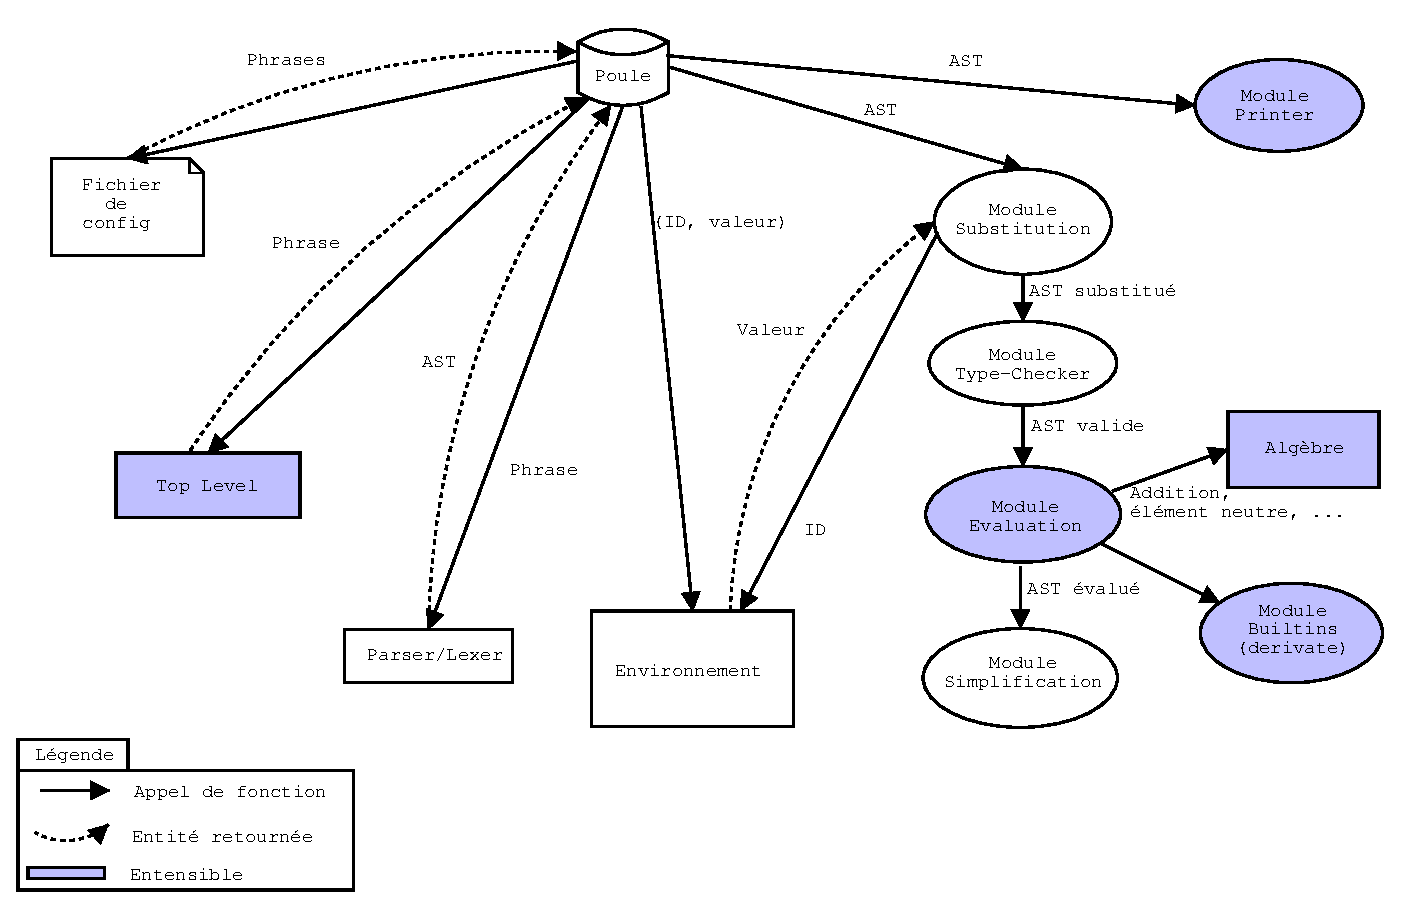
\includegraphics[angle=90]{Modules.eps}


\section{Le module {\it substitution}}

Le module {\it  substitution} a pour r\^ole de  remplacer tous les alias
contenus dans  une formule par  leur valeur.  Pour cela,  il interroge
l'environnement, interpr\`ete les r\'eponses de ce-dernier et modifie la
formule qu'il a re\c{c}ue en param\^etre.

\paragraph{}
{\bf Exemple:}

\begin{verbatim}
  poule> x = 5; 
  poule> y = x; 
  poule> y; 
  --> y = 5
\end{verbatim}

\paragraph{}
{\bf Autre exemple:}

\begin{verbatim}
  poule> R  = ]-Inf, Inf[; 
  poule> Retoile = R \ {0}; 
  poule> Retoile;
  --> Retoile = ]-Inf, Inf[ \ {0};
\end{verbatim}


\paragraph{}

L'algorithme de substitution agit ainsi.

Il parcourt l'AST et lorsqu'il arrive  sur un ID. il le remplace par sa
valeur dans  l'environemment. Si l'ID n'est  pas dans l'environnement,
il ne modifie pas la formule et poursuit son parcours de l'AST.

Lorsqu'il  arrive  sur  une  d\'efinition  de  fonction,  il  remplace
uniquement l'ensemble des variables libres.


\paragraph{}
{\bf Exemple:}

\begin{verbatim}
  poule> x  = 5; poule>  y = 10;  poule> f =  (x : R |->  x + y  : R);
  poule> f(x); --> x + 10
\end{verbatim}

\section {Le module {\it simplification}}

\subsection {Pr\'esentation}

L'algorithme  de  simplification doit  garder  la m\^eme  pr\'ecision,
c'est  \`a  dire ne  doit  pas arrondir.  Je  me  suis inspir\'e  d'un
algorithme pr\'esent\'e dans "le calcul formel sous Turbo Pascal" (voir
chapitre Etat  de l'Art). Celui-ci  \'etait par rapport \`a  une seule
variable alors  que nous voulions  le faire par rapport  \`a plusieurs
variables.Il se compose de deux parties s'appelant r\'ecursivement.

\subsection {Simplification par terme et par facteur}

Les deux algorithmes ont plus ou moins le m\^eme principe:on met l'Ast
en liste et on le  simplifie apr\`es.Pour la simplification par termes
(x+x  en  2*x par  exemple),  on utilise  une  liste  de triplets:  le
facteur, la  variable et l'exposant ($2*x^3$ en  $[(2,x,3)]$). On r\'eduit
ensuite cette liste en r\'eunissant les noeuds qui ont m\^eme variable
et  m\^eme  exposant.  Ensuite,  on  simplifie  les  facteurs  en  les
calculant  et  les variables  en  les  simplifiants  par facteurs.  La
m\'ethode de  simplification par facteur  est la m\^eme mais  la liste
n'a que deux champs (la varible et l'exposant).

\subsection {L'importance de tri}

Il est  important de  trier le r\'esultat  de ces  simplifications. Il
faut  en effet  avoir une  repr\'esentation canonique  des expressions
pour  pouvoir simplifier  toutes les  expressions. Il  faut  pour cela
mettre en  place un ordre total,  qui est ici arbitraire,  pour que le
r\'esultat d'une forme de sortie soit toujours la m\^eme quelques soit
l'entr\'ee.Par exemple $x+2$ et $2+x$ doivent donner la m\^eme chose. Cela
est important car pour  une expression comme $(x+2)*(2+x)$, on simplifie
d'abord  les deux  facteurs puis  on les  met ensembles.  Cela permet
d'avoir en sortie $(x+2)^2$.
    
\subsection {Conclusion}

Cet algorithme permet une simplification de la plupart des expressions
usuelles.Il ne simplifie  pas les expressions trigonom\'etriques comme
$sin^2(x)+cos^2(x)$. Cela est  peut g\^enant car on avait  fait le choix
d\`es le d\'epart d'un programme ne connaissant pas ces fonctions.

\section {Le module de l'environnement}

Dans  le cahier des  charges que  nous avions  \'etabli au  d\'ebut du
projet,  nous  avions \'eprouv\'e  le  besoin  de b\'en\'eficier  d'un
environnement  dans un  souci  de simplification  de l'utilisation  de
Poule et d'extensibilt\'e.

En effet,  la notion  d'environnement nous permet  de mettre  en place
plusieurs  fonctionnalit\'es.  Tout  d'abord dans  Poule, il  nous est
possible de manipuler plusieurs types de donn\'ees :

\begin{itemize}
\item Constantes math\'ematiques
\item Ensembles
\item Fonctions de bases (identit\'e sur R, ...)
\item Etc
\end{itemize}

Il nous semblait  donc tr\`es important que l'utilisateur  n'ait pas a
red\'efinir \`a chaque utilisation de Poule, les ensembles tels que R et
N ou les constantes math\'ematiques comme e et pi.

Ainsi, ces donn\'ees sont  stock\'ees dans un fichier de configuration
poule.conf. Celui ci est \'ecrit selon la syntaxe de Poule. En effet ,
cela  \'evite  \`a  l'utilisateur  d'avoir \`a  apprendre  une  deuxi\`eme
syntaxe, et cela nous permet de traiter le fichier avec l'interpreteur
de Poule.   De plus, utiliser la  syntaxe de Poule dans  le fichier de
configuration,  permet  \`a   l'utilisateur  de  pouvoir  d\'efinir  les
fonctions qu'il souhaite utiliser r\'eguli\`erement ; ce syst\`eme lui
permet  \'egalement   de  fixer  la   facon  dont  ces   fonctions  se
d\'eriveront, s'integreront, etc. En un mot, l'utilisateur peut donner
aux fonctions qu'il souhaite certaines caract\'eristiques.

\section {Le module {\it Type checkeur}}

\subsection{Contr\^ole de type sur les op\'erations}

Au cours  de la phase de  sp\'ecification de notre  projet, nous avons
d\'ecid\'e  de ne  pas permettre  les  op\'erations sur  des types  de
donn\'ees diff\'erents.  En effet, il  nous fallait d\'ecider  si nous
devions  autoriser   par  exemple  l'addition  d'un   entier  et  d'un
r\'eel. Apr\`es r\'eflexion, nous avons d\'ecid\'e d'emp\^echer ce genre
de manipulations  m\^eme si cela  peut poser probl\`eme  \`a l'utilisateur
novice de Poule.

Un "  type-checker "  parcourt donc notre  AST afin de  v\'erifier que
tous  les noeuds  ne  posent pas  de  probl\`eme de  type.  En cas  de
probl\`eme d\'etect\'e, l'utilisateur en sera inform\'e.

\subsection{Contr\^ole de type lors des appels de fonctions}

Le type-checker r\'ealise n\'ecessairement un contr\^ole de type sur les
appels  de fonctions.   Dans un  premier  temps, il  v\'erifie que  le
nombre d'arguments  que contient l'appel  de fonction est  \'egal au
nombre  de  variables  li\'ees  que  contient  la  d\'efinition  de  la
fonction.


Puis  dans un  second temps,  il v\'erifie  que la  fonction  est bien
appliqu\'ee sur son ensemble de d\'efinition.


\paragraph{}
{\bf Exemple:}

\begin{verbatim}
  poule> R = ]-Inf, Inf[; 
  poule> Retoile = R \ {0}; 
  poule> f = (x, y :  R ** Retoile |-> x / y : R); 
  poule> f(2, 1); 
  --> 2

  poule> f(2, 0); 
  --> TYPE ERROR !
\end{verbatim}

\section{Le module {\it derivate}}

Ce  module est  le  seul module  ``d'application'' impl\'ement\'e.  Il
permet de d\'eriver une expression  en utilisant les r\`egles de bases
des  op\'erateurs et  la d\'efinition  des d\'eriv\'ees  des fonctions
particuli\`eres. On peut noter que gr\^ace \`a la structure du langage
CAML et aux {\it types sommes}, la d\'escritpion du comportement d'une
deriv\'ee est  tr\`es proche de la description  mathematique, et qu'un
simple mathematicien saura, sans lire le CAML, comprendre le module et
y d\'eceler les r\`egles de d\'erivation de base. Ce dernier point est
un bon  signe quand au developpement futur  de modules d'applications,
tels que l'integration ou la r\'esolution d'\'equations.

\section{Des modules extensibles}

Nous nous sommes  attach\'es \`a r\'ealiser  un projet extensible.  Aussi, de
nombreux modules  du projet peuvent \^etre \'etendus  ou m\^eme totalement
modifi\'es sans alt\'erer le noyau du syst\`eme.



Les modules extensibles sont:
\begin{itemize}
\item Le  module de  lecture des donn\'ees. Ce  module est,
  dans  la version  du projet  que nous  rendons, un  simple top-level
  r\'ealisant   un    appel   en    boucle   \`a   la    fonction   {\it
  readline}.   Toutefois,  ce  top-level   pourrait  tr\`es   bien  \^etre
  remplac\'e par un \'editeur avec une interface graphique.  En effet,
  le top-level  se contente  de lire une suite de  caract\`eres termin\'es  
  par un retour chariot (un travail  que peut r\'ealiser simplement n'importe
  quel \'editeur).

\item  Le module {\it  printer}, qui  affiche \`a  l'\'ecran les  AST de
  poule.     Ce    module    pr\'esente   de    grandes    capacit\'es
  d'extensibilit\'e:  possibilit\'e  de  r\'ealiser  du  pretty-print,
  d'afficher  les  r\'esultats  dans  des  fichiers,  de  cr\'eer  des
  fichiers tex, ...

\item   L'alg\`ebre,  qui   d\'efinit  les   corps,  les   anneaux,  les
  op\'erations arithm\'etiques avec  lesquels le module d'\'evaluation
  va interragir.  Ce module peut \^etre enti\`erement  r\'e\'ecrit avec une
  alg\`ebre qui manipulerait des strings par exemple.

\item  Le  module  builtins,  qui  ne contient  actuellement  que  les
  fonctions de calcul des d\'eriv\'ees. L'\'elargissement de ce module
  peut  permettre de  g\'erer  les int\'egrales,  les primitives,  les
  r\'esolutions  de syst\`emes d'\'equation...   Il est  int\'eressant de
  remarquer  que ce  module  offre au  projet d'\'enormes  capacit\'es
  d'extension en ce sens qu'il est possible  d'ajouter  de  multiples  
  builtins; des ajouts qui \'etofferont les fonctionnalit\'es du projet sans 
  avoir \`a modifier des parties externes au module.
  
\end{itemize}

\section{La ligne de commande}

Lors de la  r\'edaction du cahier des charges  nous avions pens\'e que
la ligne de  commande pourrait etre dans un  petit \'editeur graphique
(en GTK ou autre).  Des probl\`emes de compilation \`a l'\'ecole et donc
de  portabilit\'e, nous  fait revenir  \`a  une bonne  vieille ligne  de
commande  dans un  terminal.  Nous  avons donc  d\'ecid\'e  de ne  pas
red\'evelopper une gestion de ligne de commande  de " a " \`a " z " afin
de ne  pas perdre  un temps pr\'ecieux.  Quelques recherches  nous ont
permis  de   d\'eterminer  que   la  commande  C   readline  repondait
parfaitement    \`a   toutes   nos    attentes.   Ainsi    dans   Poule,
l'int\'egralit\'e du code est en Ocaml except\'e le module de ligne de
commande qui est  \'ecrit en C. Ainsi, nous  b\'enficions de toutes le
fonctionnalit\'es  de  la  fonction   C  readline  dans  notre  projet
Poule.  Cette \'etape  a \'et\'e  tr\`es rapide  et nous  a  permis de
pouvoir tester d\'esormais Poule avec plus de souplesse.

\section {Int\'egration formelle}

Dans les premieres fonctionnalit\'e que nous souhaitions impl\'ementer
se   situait   la   d\'erivation.   Ensuite  nous   pensions   pouvoir
impl\'ementer l'int\'egration  formelle.  En faisant  un rapide \'etat
de  l'art  sur  ce  sujet,  nous  nous  sommes  heurter  \`a  certains
probl\`emes   de  taille.    En  effet,   les   m\'ethodes  trouv\'ees
n'\'etaient pas  r\'ealisables dans le  temps qui nous  \'etait imparti
car certaines n\'ec\'essitaient le d\'eveloppement d'un certain nombre
de sous-modules  et d'autres exigeaient  un temps de  r\'eflexion dont
nous ne disposions pas.

\chapter {P\'er\'enit\'e du projet}

\section{Evolution imm\'ediate}

\subsection{Ajout de fonctionnalit\'es}

L'ajout de  fonctionnalit\'es \`a Poule  ne pose aucun  probl\`eme en
terme  d'implementation. Il  suffit  pour cela  de  cr\'eer un  module
param\'etr\'e par  le module Ast  dans l'interpr\'eteur et  ensuite de
rajouter l'appel  \`a la fonction dans ce  m\^eme interpr\'eteur. Cela
ne prend pas plus de quelques lignes de codes.

\subsection{Changement de types de travail}

Pour l'instant Poule utilise des entiers et des flottants standards de
taille limit\'ee.  Il serait interessant de pouvoir utiliser des types
plus grands comme les BigNum, par exemple ou un type cr\'e\'e de toute
pi\`ece pour  rajouter un  module de calcul  arythm\'etique comprenant
une  factorisation   par  exemple.   Le  module  Ast   est  un  module
param\'etr\'e   par   un   module   servant   d'interface   entre   la
mod\'elisation   math\'ematique   et   l'impl\'ementation   proprement
dite.  Pour changer  le type  de travail,  il suffit  donc  de cr\'eer
l'anneau  et   le  groupe  correspondant  et  de   cr\'eer  le  module
d'interface. En changeant la cr\'eation du module d'Ast, on change les
types utilis\'es dans  tous le programmes. On peut  imaginer la m\^eme
chose pour le corps et l'anneau de travail m\^eme si l'int\'er\^et est
moins \'evident.


\section{Evolution \`a moyen terme}

\subsection{Changement de types au cours de l'ex\'ecution}

Il serait int\'eressant de pouvoir  changer le type de travail pendant
l'ex\'ecution  du programme.  Par exemple,  on voudrait  travailler en
marche "normale" puis  passer en grands entiers puis  revenir avec des
entiers normaux. Il  faut pour cela charger du  code dynamiquement, ce
qui est  possible en ocaml.   En effet, notre projet  fonctionnant \`a
base de foncteurs, il faudrait cr\'eer tous les modules pouvant \^etre
utilis\'es, ce qui  n'est pas envisageable. POur cela,  il faut mettre
en place un module comprenant tous les autres modules instanci\'es. Ce
module  serait   charg\'e  \`a  l'aide  d'une   commande  ("load"  par
exemple).  Cela pose  un probl\`eme  car l'environnement  serait alors
perdu  car  les  types  seraient  alors  diff\'erents.   La  solution,
envisag\'ee  pendant  le d\'eveloppement  mais  abandonn\'ee faute  de
temps, est faire un Ast sans type, avec des strings pour repr\'esenter
les  entiers  puis de  le  passer  quand on  en  a  besoin  en un  Ast
typ\'e.  Cela  enteine  de  l\'eg\`ere  modification  \`a  faire  dans
l'environnement: il faudrait typ\'e  l'Ast que l'on retourne lors d'un
appel \`a l'environnement.

\subsection {Changement de groupe et d'anneau}

Il serait  int\'eressant de  pouvoir changer le  corps et  l'anneau de
travail pendant l'ex\'ecution. On  peut imaginer par exemple passer du
corps  des r\'eels  \`a Z/2Z  ou un  autre corps  fini. Pour  cela, il
faudrait mettre en place la solution ci-dessus. On peut aussi imaginer
que l'on puisse  passer le corps et l'anneau  de travail aux fonctions
qui les  utilisent, et on pourrait  alors se passer  de l'interface et
instancier les objets de classe anneau ou corps et les utiliser.

\section{Evolution \`a long terme}

Ces  \'evolutions changent  la grammaire  et donc  l'Ast  mais peuvent
\^etre  mises  en place  plus  ou  moins  facilement.On peut  imaginer
rajouter  un syst\`eme  de r\'esolution  d'\'equations. Pour  cela, il
faudrait rajouter une r\`egle du genre "$Exp = Exp$".  En rajoutant cela
dans l'Ast, on peut  ainsi obtenir une r\'esolution d'\'equation voire
de  syst\`eme d'\'equations  .On  peut aussi  imaginer introduire  une
sorte de langage de programation du m\^eme genre que mapple, incluant,
pourquoi pas, la gestion des listes en plus de celles des variables.

\section{Conclusion}

Il  est  donc  possible  de  faire  progresser  Poule  en  gardant  la
mod\'elisation proche  des math\'ematiques. Ces  modifications peuvent
\^etre  superficielles  ou alors  plus  profondes. Cette  architecture
permettant l'\'evolution future du projet  fait de ce projet une bonne
base pour le d\'eveloppement d'une station de calcul formel respectant
l'architecture des math\'ematiques.

\chapter {Objectifs}

A  l'issue  du developpement  de  Poule,  certains  objectifs ont  ete
atteints, d'autres  non. Mais ces derniers  restent faisables grace
\`a notre  modelisation, qui  permet comme nous  l'avons deja  dit une
grande extensibilite.

\section {Les objectifs atteints}

Cette extensibilte  est un  objectif qui nous  etait cher, car  de lui
decoulait la  perennite du projet.   Cette objectif a ete  atteint car
les  problemes souleves  en  fin de  developpement  peuvent tous  etre
resolus avec un  minimum de modifications du code.  Poule repose comme
prevu sur  un systeme d'algebre  qui permet egalement  a l'utilisateur
une grande extensibilite puisque chaque il peut redefinir le corps sur
lequel il souhaite travailler. Le controle des types est operationnel,
la  substitution  des  variables  egalement,  ce qui  nous  permet  de
presenter  une evaluation  d'expression  finie. Au  niveau formel,  la
simplification des  expressions ainsi que le calcul  des derivees sont
implementes et fonctionnels.

\section {Les objectifs non atteints}

Parmi  les objectifs  que  nous  n'avons pas  pu  atteindre se  trouve
diverses fonctionnalit\'es que nous n'avons pu impl\'ementer, faute de
temps.

Beaucoup d'objectifs n'ont pas \'et\'e atteind faute de temps, la mise
en place  de la mod\'elisation  ayant \'et\'e plus longue  que prevue.
Ainsi la repr\'esentation graphique n'est actuellement pas disponible,
cette   fonctionnalit\'e  ne   pouvant  \^etre   mise  qu'en   fin  de
developpement.   Au   niveau  calcul  formel,   la  factorisation,  le
developpement,  la r\'esolution d'equations  et l'integration  ne sont
pas operationnels.  Contrairement \`a  ce qui est expliqu\'e plus haut
sur  les raisons  qui nous  ont empech\'e  d'implementer l'integration
formelle,  les   autres  fonctionnalites  sont   implementables  assez
rapidement.

Ainsi  les  objectifs qui  nous  tenaient  \`a  coeur et  qui  etaient
necessaires  pour  garantir  la  p\'er\'ennit\'e du  projet  sont  eux
atteints.


\end{document}